\documentclass[letterpaper,twocolumn,10pt]{article}
\usepackage[utf8]{inputenc}
\usepackage{usenix,epsfig,hyperref}
\usepackage{amsmath,amssymb}
\usepackage{booktabs}
\usepackage{graphicx}
\usepackage{microtype}
\usepackage{xcolor}
\usepackage{caption}
\usepackage{url}
\usepackage{xspace}

\hypersetup{
  colorlinks=true,
  linkcolor=black,
  citecolor=black,
  urlcolor=blue!60!black
}

\newcommand{\code}[1]{\texttt{#1}}
\newcommand{\opcode}[1]{\texttt{#1}}
\newcommand{\sysflag}[1]{\texttt{#1}}
\newcommand{\iouring}{\texttt{io\_uring}\xspace}
\newcommand{\s}{\ensuremath{\mathcal{S}}\xspace}
\renewcommand{\r}{\ensuremath{\mathcal{R}}\xspace}

\begin{document}

\date{}

\title{\Large \bf Covert Channels in the \texttt{io\_uring} Runtime}

\author{
{\rm Joshua Gillett}\\
Harvard University
}

\maketitle
\thispagestyle{empty}

\section*{Abstract}
Linux's \iouring subsystem is an asynchronous interface used to bypass the context-switching overhead of I/O system calls. \iouring uses shared-memory ring buffers between the user and the kernel to provide performant I/O operations. However, this still entails some amount of syscalls. In order to push a submission queue to the kernel, a participant process must call \code{io\_uring\_enter()}. If, as an ambitious systems programmer, you want to avoid this, \iouring exposes the option for a dedicated polling kthread (\code{SQPOLL}) that drains submissions without entering the calling task. Prior side-channel work on \iouring has focused on the contention against the storage device or the PCIe bus. We instead ask whether the runtime itself---its scheduler, registered-resource tables, and documented cross-ring primitives---can be used to communicate between two processes that share no permitted IPC.

We answer this question in the affirmative with three different layers of required capability for the attacker. (1)~When two rings can share an \code{SQPOLL} backend via \code{IORING\_SETUP\_ATTACH\_WQ}, a single shared kernel polling loop is enough to carry $\approx86$ bits/sec at a five-fold cross-validated bit error rate (BER) of $0.09\%$ on a commodity laptop. We attribute this signal directly to the \code{SQPOLL} inner-loop scan via a Cohen's-$d$ versus ring-fan-in sweep. (2)~When the rings cannot share an \code{SQPOLL} backend, but both call \code{IORING\_REIGSTER\_FILES} on a common backing \code{struct file} (e.g., \code{/dev/null}), a sender can cause contention in \code{IORING\_REGISTER\_FILES\_UPDATE} by modulating the \code{f\_ref.refcnt} cache line, for which a receiver can load on every \code{io\_file\_get\_fixed} call. Repetition coding allows this channel to transmit $\approx0.625$ bits/sec with a BER of $0.08$. (3)~When neither shared \code{SQPOLL} nor common registered resources are available, but the sender is able to hold a file descriptor to the receiver's ring, \code{IORING\_OP\_MSG\_RING} provides a documented and kernel-approved cross-ring CQE delivery primitive that achieves a BER of $0.008$ at $\approx18$ bits/sec.

\section{Introduction}
Compared to \texttt{epoll/aio}, \iouring removes a per-operation syscall trap by sharing two ring buffers between the kernel and a process, a Submission Queue (SQ) and a Completion Queue (CQ) \cite{axboe2019efficient}. With \texttt{IORING\_SETUP\_SQPOLL}, the kernel additionally spawns a dedicated kthread to poll the SQ and write the CQ on the user's behalf, eliminating syscall traps on the hot path entirely. This design has made \iouring popular in high performance database engines, network proxies, and workloads that are generally bottlenecked by syscall overhead, and is increasingly enabled in multi-tenant cloud environments where co-resident, mutually distrustful processes share the same kernel \cite{jasny2025iouring, kalmbach2020io_uring}.

Use in said co-resident environments raises the security question, that has to our knowledge, not been answered for the runtime layer of \iouring. There is prior work, recently, on covert channels through the storage side of \iouring--- Juffinger et al. demonstrate a covert channel that explots PCIe-bus contention provoked by unprivileged \iouring I/O--- but if a covert channel can be constructed by modulation in the runtime, storage-class mitigations for this covert channel cannot prevent disallowed communication \cite{juffinger2025secret}.

Our project, thus, asks if two isolated processes can communicate covertly through \iouring's runtime without shared user-space memory, IPC, and without touching the block-layer storage. The answer turns out to be that it is largely dependent on the system administrator's sandboxing policy since different elements, and that the possibility mostly remains under a restrictive policy, but degrades. We, therefore, organize our results into three layers of attacker capabilities.

\paragraph{Channel I: shared \code{SQPOLL} backend.} If both processes are able to create rings with \code{IORING\_SETUP\_ATTACH\_WQ}, they will share a single \code{SQPOLL} kthread. The kthread's hot loop will then iterate over every attached ring and process its SQ tail. A process can thus send a burst of \code{IORING\_OP\_NOP} operations on one ring to measurably extend the period between visits to the other process's SQ. We obtain $\approx 86$ bits/sec at a 5-fold cross-validated BER of $0.09\%$ with $N=2$ attached sender rings, a $4$-ms symbol window, and a Fisher LDA decoder over five per-window features. We confirm that the channel is internal to \code{SQPOLL} by sweeping the number of attached rings $N \in \{1,2,4,6,8 \}$ and measuring the magnitude of the Cohen's $d$ on the receiver's per-window count of issued NOPs and find that it increases monotonically from $-8.30$ to $-16.97$ before saturating at $N \geq 6$ and giving Pearson $r = -0.53$ with permutation $p = 0.043$.

\paragraph{Channel II: registered-files cache-line bouncing.} Removing \code{ATTACH\_WQ} collapses Channel I across testing. The exception is in a registed-files harness in which the sender churns its fixed-file table via \code{IORING\_REIGSTER\_FILES\_UPDATE}. A kernel-source audit found that the per-\code{struct file} atomic refcount line (\code{f\_ref.refcnt}) as the only candidate carrier that is touched on both sides of communication. To turn this audit into an empirical claim at covert communication, we ran a repetition-coded $K$-sweep at $K \in \{1,2,4,8,16,32\}$ with a $50$-ms symbol window. The receiver reaches a mean soft BER of $0.080$ at $K=32$ and has zero errors on $32$ super-symbols in the best of three trials, but has throughput of $0.625$ bits/sec.

\paragraph{Channel III: \code{IORING\_OP\_MSG\_RING} CQE delivery} \code{IORING\_OP\_MSG\_RING} is a documented opcode that lets a sender ring post a CQE on a target ring that it holds a file descriptor for. With independent \code{SQPOLL} kthreads and no registed resources, modulating the rate of inbound \code{MSG\_RING} deliveries on the receiver's CQ ring perturbs its NOP-timing loop enough that the LDA decoder can decipher a message trivially. We measure $K = 1$ BER $\approx 0.008$ at $\approx18$ bits/sec across three trials. The attacker's only required capability beyond being able to setup \iouring is possession of a file descriptor to the victim's ring which is plausible via the common ancestor process \code{SCM\_RIGHTS} or through some other form of communication.

The rest of the paper is organized as follows. We first review the \iouring kernel mechanisms our channels exploit, state our threat model, and describe the common methodology of the channels. We then present the three channels in increasing order of sandbox restrictiveness. Finally, we discuss mitigations, related works, limitations, and future work.

\section{Background}
\label{sec:background}
\subsection{The \iouring interface}
\iouring is the third-generation of Linux asynchronous I/O interfaces, introduced by Jens Axboe in 2019 \cite{axboe2019efficient}. A user process creates a ring with \code{io\_uring\_setup(2)}, which returns a file descriptor whose \code{mmap} regions back two queues: the SQ into which the user can write Submission Queue Entries (SQEs), and the CQ, on which the kernel posts Completion Queue Entries (CQEs). On a default ring, each SQE is delivered to the kernel via an \code{io\_uring\_setup(2)} syscall.

The runtime also supports a number of optional setup flags that change how, when, and by whom the SQ is drained. The two relevant to this work are as follows.
\begin{itemize}
    \item \code{IORING\_SETUP\_SQPOLL}, which spawns a kernel polling thread to watch the SQ tail and submit work itself, so user code never has to call \code{io\_uring\_enter} on the hot path. By default the kernel spawns one such kthread per ring with this flag.
    \item \code{IORING\_SETUP\_ATTACH\_WQ}, which causes a new ring to be attached to an existing ring's \code{SQPOLL} backend rather than spawning its own. All rings sharing a backend are placed within a \code{io\_sq\_data} list and are drained by one kthread.
\end{itemize}
\iouring additionally exposes a registered-resources mechanism. \code{io\_uring\_register(2)} with \code{IORING\_REGISTER\_FILES} pins an array of file descriptors into a per-ring fixed-file table, after which an SQE can refer to a slot by index rather than by file descriptor to avoid \code{fget} and \code{fput} latency. \code{IORING\_REGISTER\_FILES\_UPDATE} swaps the individual slots without re-registering the entire table. A symmetric mechanim exists for buffers in \code{IORING\_REGISTER\_BUFFERS}. Finally, the cross-ring opcode \code{IORING\_OP\_MSG\_RING} lets one ring post a CQE on a target ring whose file descriptor it possesses \cite{axboe_msg_ring}.

\subsection{Attack surface}
The standard IPC protocol for Linux--- pipes, sockets, signals, etcetera--- is common for a security policy in a multi-tenant environment to account for. \iouring's runtime introduces several new mediators that do not necessarily come to mind for a sandbox policy writer: a shaed kernel polling thread, a per-ring registered-resource table whose slots may alias to same backing \code{struct file}, and a documented ring messaging opcode. Each has a kernel-side mechanism by which one ring's behavior can be observed by another ring without invoking IPC.

Prior side-channel work has examined \iouring from the storage dvice or the PCIe interconnect, but the runtime also holds distinctive design \cite{juffinger2025secret}. Our work treats the runtime layer as a first-class attack surface and asks how much bandwidth and how clean a BER each analyzed runtime feature can carry under realistic, non-cooperative assumptions on shared state.

\subsection{Covert timing channels and capacity}
Lampson's confinement-problem framing of covert channels treats them as any communication mechanism not explicitly intended for communication \cite{lampson1973note}. Our channels fit this strictly since the sender modulates a kernel-mediated quantity--- a scan-loop visit period, a refcount cache-line state, or a CQ-arrival rate--- that the receiver can observe through timing.

For analysis, we model each channel as a binary symmetric channel (BSC) whose crossover probability is the per-window BER $p$. The Shannon capacity is,
\begin{align*}
    C(p) &= 1 - H_2(p) \\
    H_2(p) &= -p \log_2 p - (1- p) \log_2 (1-p)
\end{align*}
in bits per channel use. Any non-degenerate $p < \frac{1}{2}$ gives $C(p) > 0$, so the channel is information-theoretically useable regardless of how poor the per-symbol decision is. We explot this explicitly with repetition coding: a length-$K$ repetition code transmits each information bit $K$ times at a rate of $1/K$, and hard-decision majority voting reduces the BER towards zero exponentially in $K$ by a Chernoff bound. For $p=0.367$, the $K=1$ BER of our second channel, the analytic hard-majority $p_K$ satisfies $p_4 \approx 0.34$, $p_{16} \approx 0.13$, $p_{32} = 0.058$, $p_{128} \approx 2.8 \times 10^{-3}$. Repetition is far from capacity-approaching since the $C(0.367) \approx 0.052$ ceiling at our $50$-ms window corresponds to $\approx 1.04$ info-bits/sec, an order of magnitude above what we deliver at $K=32$, but it is the simplest possible code and serves our existence claim. We discuss capacity-approaching follow-ups in Section X.X. % ADD SECTION HERE

\section{Threat Model}
We consider two co-resident mutually distrustful processes \s (sender) and \r (receiver) on a single Linux host. Both can call \code{io\_uring\_setup(2)} and submit SQEs, but neither has any sanctioned IPC channel to the other. The adversary controls \s and seaks to leak data to a co-resident \r, which is also controlled by the adversary, without being recorded by some sandbox policy as performing IPC.

For each channel, we state explicitly what additional state, if any, \s and \r must arrange to share at ring-creation time. Whether each precondition is realistic depends on the sandbox policy--- e.g. \code{ATTACH\_WQ} is plausible inside a single container's \iouring pool but can be denied by seccomp, sharing a \code{struct file} is given for any globally shared inode (\code{/dev/null} is particularly convenient), but can be disallowed by mount or namespace separation, a passed ring file descriptor is plausable across descendants of a common process or via \code{SCM\_RIGHTS} but can be revoked by sandbox API decisions.

We notably do not consider hardware-level side channels such as cache prime+probe \cite{percival2005cache, yarom2014flushreload,liu2015lastlevel}, branch-predictor channels \cite{evtyushkin2018branchscope}, or the particularly famous speculative-execution channels \cite{kocher2019spectre, lipp2018meltdown}, and instead focus our threat model on the runtime of \iouring. Where our channel interacts with hardware, we note this interaction explicitly, as in Section~\ref{sec:ch2attribution}. % ADD SECTION HERE

\section{Methodology}
This section describes the parts of the experimental design that are common to all three channels: how the sender modulates a binary signal, how the receiver instruments per-window features, how they are decoded, and how observed effects are attributed back to specific kernel mechanisms.

\subsection{Symbol modulation}
The sender encodes one bit per symbol window of width $W$ milliseconds. In bit-$1$ windows, it ``hammers'' a configurable kernel operation (NOP storm, registered-file update churn, or \code{MSG\_RING} flood) at a configured rate and in bit-0 windows it goes idle. The receiver runs its own probe loop at teh same window width with epoch-aligned start times derived from \code{CLOCK\_MONOTONIC}. Both sides emit per-window CSV records keyed by window index. A short payload prefix (``\code{10101001110}'' is our canonical 11-bit pattern for the \code{ATTACH\_WQ} channel and longer pseudo-random patterns are used for the repetition-coded channel) repeats \code{LOOPS} times to amortise the per-trial sync cost.

\subsection{Receiver instrumentation}
The receiver issues its own \code{IORING\_OP\_NOP} (or, for Channel II, \code{IORING\_OP\_NOP} with the correct \code{nop\_flags}, or for the buffer-register variant of Section X.X, \code{IORING\_OP\_READ\_FIXED}) and times each submit/reap iteration with \code{rdtsc}. For each window, the receiver records:% add section here
\begin{itemize}
    \item \code{samples}, the number of complete probe iterations.
    \item \code{median\_cycles}, \code{p90\_cycles}, \code{p99\_cycles},
    \item \code{mean\_cycles},
    \item \code{max\_cycles}.
\end{itemize}
These features are saved to a CSV which the offline analyzer can read.

\subsection{Decoder: Fisher LDA}
Originally, a single feature and fixed-threshold rule decoder was used, but this performs poorly on \code{median\_cycles}. Thus, we moved to a Fisher Linear Discriminant-Analysis (LDA) over the five-dimensional feature vector \cite{fisher1936lda}. LDA picks the direction $\mathbf{w} \propto \sum_{w}^{-1} (\bar{\mathbf{x}}_1 - \bar{\mathbf{x}}_0)$ that maximizes between-class variance over within-class variance, projects each window onto $\mathbf{w}$, and classifies by sign relative to the midpoint. To avoid optimistic bias on small payloads, we score every cell by 5-fold stratified cross-validation: five times we hold out a fifth of the windows, fit on the remaining four-fifths, and report teh held-out BER. The LDA-CV-BER reported throughout the paper is the mean of these five held-out folds.

\subsection{Effect size and significance tests}
The headline number of any covert channel is its BER, but two additional summaries help us reason about why a channel works. We use Cohen's $d$ on each per-window feature \cite{cohen1988statistical},
\begin{align*}
    d_f = \frac{\bar{x}_{f,1} - \bar{x}_{f,0}}{s_{p,f}},
\end{align*}
where $s_{p,f}$ is the pooled standard deviation, as our headline effect-size metric. $|d| \geq 0.8$ is conventionally ``large.'' We report $d$ on samples as the cleanest descriminator under \code{ATTACH\_WQ}, and on per-feature panels for the attribution sweeps. Cell-level statistical significance is reported via two-twailed permutation tests on either Pearson $r$ (for the $N$-th sweep) or paired-trial means.

\subsection{Falsifiers for kernel attribution}
Once a channel is shown to exist with low enough BER to be useful, the next question we ask is which kernel mechanism carries said bits. Attribution is harder than measurement becasue the kernel's hot path runs many primitives concurrently and the candidate carriers (a mutex, a per-task spinlock, an atomic refcount, an allocatior partial-list lock) cannot be turned off individually for a given hot path. Our methodology, applied explicitly in Section X.X and X.X, is as follows.
\begin{itemize}
    \item Read the kernel source (mirrored under \code{deps/kernel\_io\_uring/}, all citations against \code{torvalds/linux v6.13}), and enumerate every synchronization primitive that either side of the channel touches.
    \item For each candidate primitive $P$, design a binary in which the sender's hot churn is the smallest possible workload that would amplify $P$ if $P$ were the carrier (e.g. \code{dup/close} for \code{current->files->file\_lock} and \code{getpid()} for the bare-syscall noise floor).
    \item Run all variants under the same receiver, payload schedule, CPU pinning, and decoder, and record their BER under repetition coding.
    \item Tabulate. The variant whose BER is best after holding the receiver fixed points to the carrier, by contrast with the worst variant ruling out an alternative carrier which was not amplified.
\end{itemize}

\subsection{Hardware environment}
All experiments reported in this paper run on a single Fedora 42 laptop with an Intel Core i7-8650U (8 logical cores, single NUMA node, 1.9 GHz base clock), kernel 6.19. We pin the sender thread, receiver threa,d and \code{SQPOLL} kthread to distinct logical cores via \code{sched\_setaffinity} and \code{IORING\_SETUP\_SQ\_AFF}. We also use a vendored \code{liburing} build under \code{deps/liburing-install} so that the binary ABI is stable across runs. While the hardware is admittedly modest, we expect that a industry-scale server to have cleanly higher absolute capacities and lower BERs. We cite the implication of the limitation explicitly in Section X. % add section here

\section{Channel I: Shared \code{SQPOLL} Backend}
\label{sec:ch1}
\subsection{Mechanism}
When a ring is created with \code{IORING\_SETUP\_ATTACH\_WQ}, it joins an existing ring's \code{io\_sq\_data} list. Inside \code{io\_sq\_thread} (\code{io\_uring/sqpoll.c}) the polling kthread runs a round-robin loop:
\begin{verbatim}
list_for_each_entry(ctx, &sqd->ctx_list, ...)
        __io_sq_thread(ctx, ...);
\end{verbatim}
At each visit to a context, the kthread reads the SQ tail, copies SQE bytes from the user-mapped ring into kernel state, dispatches each SQE, and posts CQEs. The wall-clock time spent inside one context's visit directly delays the next visit to every other context on the same list. From the receiver's point of review, the period between successive visits to its own ring is the per-NOP service rate.

\subsection{Implementation details}
We implement this channel as the binary, \code{attached\_multi}, that takes \code{--num-sender-rings N} as an argument. A base ring is created with \code{IORING\_SETUP\_SQPOLL} and \code{IORING\_SETUP\_SQ\_AFF} so that the kthread is pinned to a fixed logical core. The sender then creates $N$ additional rings with \code{IORING\_SETUP\_ATTACH\_WQ} pointing to the base ring's file descriptor, and the receiver creates one such ring in the same way. All $N+2$ rings are on the same \code{io\_sq\_data} list and therefore share a single kthread. In bit-1 windows, each sender submits $I$ in-flight \code{IORING\_OP\_NOP} SQEs, across its $N$ rings. In bit-0 windows, it drains said SQ. The receiver's probe loop is unchanged from the single-ring case.

\subsection{Cell-grid sweep}
We swept the Cartesian product $N \in \{1,2,4\} \times W \in \{10,20,30,50\} \text{ ms } \times I \in \{100,200\}$ SQEs per ring and recorded the LDA-CV-BER and wall-clock bits/sec for each triple. The Pareto-optimal cell--- dominant on both axes--- was $N=2$, $W = 10$ms, $I = 100$, at $56.7$ bits/sec and LDA-CV-BER $= 0.000$. Below $W = 10$ms, we expect that we hit the \code{SQPOLL} wakeup-jitter on the CPU and above $W=50$, we simply lose throughput.

\subsection{\texorpdfstring{Sub-$10$ ms symbol sweep}{Sub-10 ms symbol sweep}}
To push this cell finer, we ran a sub-$10$ ms sweep with $W \in \{4,6,8,10,12,15\}$ ms at $N=2$, $I = 100$. Three trials at each cell exposes two candidates as superior ($W = 4$ and $W = 6$). We then, ran $8$ trials at each. Table~\ref{tab:sub10} summarizes the results of this. 

The Pareto-optimal cell is, therefore, $W = 4$ ms, where the receiver manages enough probe iterations per window to separate the classes. Thus, we adopt ($N = 2$, $W = 4$ms, $I = 100$) as the configuration for Channel I. Across $8$ trials with $5$-fold CV each, the cofiguration emits a single bit error on only one fold, for an aggregate LDA-CV-BER of $0.0009$. Wall-clock throughput is $85.9$ bits/sec including a $1$-second sync window.
\begin{table}[t]
\centering\small
\caption{Sub-$10$ ms symbol sweep at $N=2$, $I=100$ on \code{attached\_multi}. ``LDA CV BER'' is the mean $\pm$ std across all five folds of all $n$ trials. ``$\#0$'' counts trials whose 5-fold CV BER was identically zero out of $n$.}
\label{tab:sub10}
\setlength{\tabcolsep}{4pt}
\begin{tabular}{rrrlrr}
\toprule
$W$ (ms) & $n$ & $|d|$ on \code{samples} & LDA CV BER & bits/s & $\#0$ \\
\midrule
$4$  & 8 & $14.4 \pm 2.3$  & $0.0009 \pm 0.0026$ & $85.9$ & $7$ \\
$6$  & 8 & $11.2 \pm 1.7$  & $0.0028 \pm 0.0039$ & $73.3$ & $5$ \\
$8$  & 3 & $12.3 \pm 2.1$  & $0.0026 \pm 0.0044$ & $64.0$ & $1$ \\
$10$ & 3 & $11.8 \pm 5.2$  & $0.0026 \pm 0.0044$ & $56.7$ & $1$ \\
$12$ & 3 & $17.3 \pm 3.6$  & $0.0000 \pm 0.0000$ & $50.9$ & $3$ \\
$15$ & 3 & $\phantom{0}5.95 \pm 2.8$ & $0.0304 \pm 0.0305$ & $44.2$ & $0$ \\
\bottomrule
\end{tabular}
\end{table}

\subsection{Attribution}
The throughput gain and low BER are not yet evidence that the channel runs through the \code{SQPOLL} portion of the runtime, because adding rings increases both kernel-side load and CPU-side cache pressure. To attribute the signal directly to the kthread's per-pool inner loop, we hold the operating point fixed at $W = 100$ms and sweep $N \in \{1,2,4,6,8\}$ with three trials per cell.

Our hypothesis is as follows. If the carrier is the \code{SQPOLL} inner-loop scan, the magnitude of Cohen's $d$ on the receiver's \code{samples} feature should change monotonically with $N$ before saturating around the value of $N$ at which the inner-loop scan itself becomes the bottleneck (rather than per-ring SQE processing). The competing hypothesis that the leak is L1/L2 cache or scheduler contention around \iouring but not inside it predicts a mostly flat or noisy curve.

\begin{figure}[t]
\centering
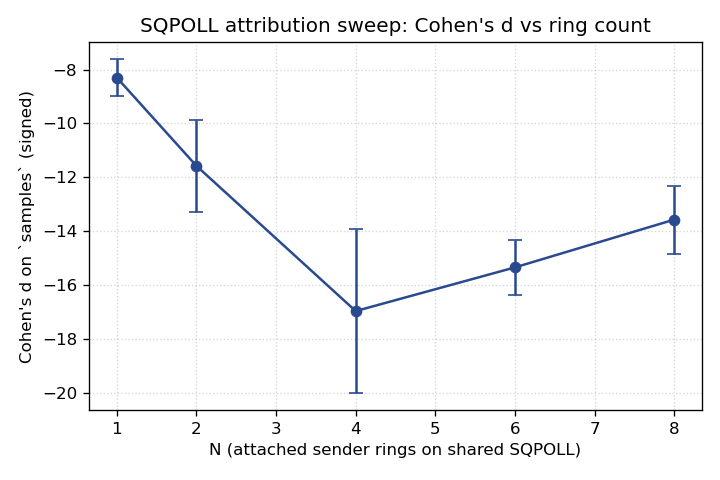
\includegraphics[width=0.95\columnwidth]{ch1_attribution.png}
\caption{Cohen's $d$ on the receiver's \code{samples} feature versus the number $N$ of attached sender rings funnelled into one shared \code{SQPOLL} backend (mean $\pm$ std over $3$ trials per cell). The aggregated correlation has Pearson $r = -0.532$, Spearman $\rho = -0.600$, and two-tailed permutation $p = 0.043$ ($n_\text{perm} = 10000$).}
\label{fig:attribution}
\end{figure}

Figure~\ref{fig:attribution} shows the results of this experiment. The signed Cohen's $d$ on \code{samples} drops from $-8.30 \pm 0.69$ at $N = 1$ to $-16.97 \pm 3.06$ at $N =4$ and then recovers to $-13.57 \pm 1.26$ at $N= 8$. The saturation around $N = 4$ and recovery beyond are consistent with two effects. At $N \geq 4$, the inner-loop scan itself is the dominant cost (so adding rings no longer widens the gap), and at $N = 8$ the sender thread's CFS scheduler across rings limits the effective per-ring submission rate. We did not push $N$ further because of the limitations of the 8-logical-core CPU that was used.

The aggregated 15-cell statistic with Pearson $r = -0.532$, Spearman $\rho = -0.600$ , two-tailed permutation $p = 0.043$ at $n_\text{perm} = 10000$ is significant at $\alpha = 0.05$. We read this as direct evidence that the carrier must be internal to the \code{SQPOLL} runtime, since the rings share no other state in this experiment.

\section{Channel II: Registered-Files Cache-Line Bouncing}
A natural follow-up to the first channel is whether a covert channel in the \iouring runtime can exist without \code{ATTACH\_WQ}. The simple version of this question has a clean answer in the negative, but finding the more interesting positive answer required a kernel-source audit and a five-binary falsifier table, which we present in this section.

\subsection{Sweep without \code{ATTACH\_WQ}}
We first test the simple question with eight variants run at the same canonical cell of $W = 100$ms, $I = 200$, payload $10101001110$, \code{LOOPS}$=12$, with $1$ second syncs and in $5$ trials each. Each variant differs only in what the sender modulates, and the receiver's probe loop and LDA decoder remain unchanged from Section~\ref{sec:ch1}. Table~\ref{tab:trackB} summarizes these results.

We note from this that CPU-sharing alone (\code{independent\_pair}, same-CPU) and allocator pressure alone (\code{many\_ring\_pressure}, $N = 8$) were unable to produce a measurable signal. The only exception to our trials is that \code{regfile\_pair}, our test with register-update on registered files achieves $|d| = 0.26 \pm 0.13$, which is $3\times$ the next-best variant. The signal is too small to decode but is well above the noise floor of every other variant, and so deserves a focused follow-up.

\begin{table*}[t]
\centering\footnotesize
\caption{No-\code{ATTACH\_WQ} sweep with $5$ trials each. \code{attached\_pair\_ctrl} retains \code{ATTACH\_WQ} as a positive control.} 
\label{tab:trackB}
\begin{tabular}{lcccccc}
\toprule
Variant & $n$ & $|d|$ \code{samples} & $|d|$ \code{p99} & uni-test BER & LDA CV BER & Verdict \\
\midrule
\code{attached\_pair\_ctrl} (with \code{ATTACH\_WQ}) & 5 & $8.73 \pm 1.14$ & $2.48 \pm 1.25$ & $0.024 \pm 0.018$ & $0.009 \pm 0.003$ & strong (control) \\
\code{independent\_pair}, different-CPU \code{SQPOLL} & 5 & $0.06 \pm 0.07$ & $0.13 \pm 0.15$ & $0.455 \pm 0.039$ & $0.455 \pm 0.044$ & no channel \\
\code{independent\_pair}, same-CPU \code{SQPOLL} & 5 & $0.08 \pm 0.11$ & $0.08 \pm 0.07$ & $0.519 \pm 0.044$ & $0.550 \pm 0.040$ & no channel \\
\code{many\_ring\_pressure} ($N=8$), different-CPU & 5 & $0.10 \pm 0.09$ & $0.14 \pm 0.07$ & $0.481 \pm 0.038$ & $0.448 \pm 0.035$ & no channel \\
\code{many\_ring\_pressure} ($N=8$), same-CPU & 5 & $0.08 \pm 0.11$ & $0.05 \pm 0.14$ & $0.501 \pm 0.032$ & $0.515 \pm 0.044$ & no channel \\
\code{regfile\_pair}, churn rate $1/64$ & 5 & $\mathbf{0.26 \pm 0.13}$ & $0.19 \pm 0.17$ & $0.343 \pm 0.106$ & $0.432 \pm 0.052$ & marginal \\
\code{regfile\_pair}, no update churn & 5 & $0.14 \pm 0.09$ & $0.10 \pm 0.10$ & $0.424 \pm 0.083$ & $0.451 \pm 0.068$ & no channel \\
\code{hotpath\_pair}, default \code{task\_work} & 5 & $0.10 \pm 0.06$ & $0.08 \pm 0.14$ & $0.491 \pm 0.050$ & $0.510 \pm 0.051$ & no channel \\
\bottomrule
\end{tabular}
\end{table*}

\subsection{Kernel-source audit}
From reading \code{io\_uring/register.c}, \code{io\_uring/rsrc.c}, \code{fs/file.c}, and \code{fs/file\_table.c} at \texttt{v6.13}, we enumerate every lock and atomic on the call chain of the sender's \code{io\_uring\_register\_files\_update} syscall and the receiver's \code{IORING\_OP\_NOP} with \code{IOSQE\_FIXED\_FILE} set. Eleven primitives appear upon these paths. We list the following four with the strongest prima-facie case for being the carrier.
\begin{description}
    \item[(a) \code{ctx->uring\_lock}] is held by the sender for the duration of the registers-update syscall and by the receiver's \code{SQPOLL} kthread during SQE submission. However, each ring has its own \code{ctx->uring\_lock}. Thus, we rule it out by inspection.
    \item[(b) \code{current->files->file\_lock}] is the per-task spinlock that guards file-descriptor table mutations. By inspection, it is taken on \code{dup}, \code{close}, and on \code{\_\_alloc\_fd} write paths. It is not taken on \code{fget}, which uses RCU. Neither the sender's register-update path nor the receiver's NOP path takes \code{file\_lock} in steady state, but this hypothesis is quite natural so we explicitly build a falsifier to test it.
    \item[(c) \code{kmem\_cache\_node->list\_lock}] for the \code{kmalloc-32} cache which backs \code{struct io\_rsrc\_node} and the per-CPU \code{pcp\_lock} for the page allocator. The sender's \code{kzalloc(sizeof(io\_rsrc\_node))} inside \code{io\_register\_files} hits this slab and acquires the per-NUMA \code{list\_lock}. The receiver's \code{io\_kiocb} allocations come from a different \code{kmem\_cache}, so direct \code{list\_lock} is not possible, but both caches share the underlying page allocator. Heavy churn from the sender can, thus, drain the per-CPU PCP free list and force the next allocation on any CPU in the same NUMA zone to refill from the buddy allocator under \code{zone->lock}. This is, therefore, a candidate.
    \item[(d) \code{file->f\_ref.refcnt}] is simply an \code{atomic64\_t} inside \code{struct file} which is incremented by \code{fget} and decremented by \code{fput} through full-barrier RMWs. When all \code{dup}s in our churn pool alias to the same \code{struct file} for \code{/dev/null}--- they do, by construction--- every register-update produces two RMWs on the same cache line. If the receiver's NOP path also reads \code{f\_ref}, MESI coherence will bounce the line between the two CPUs. This is clearly also a candidate.
\end{description}
We expect (d) to be the strongest candidate since it it is the only primitive on the audit whose backing memory is the same on both sides. We thus, also taking into account what we believe to be a small UX bug in \iouring, test these under repetition coding.

\subsection{Repetition-coding empirical results}

At $W = 50$ms, \code{regfile\_nop} (the same test as \code{regfile\_pair} with churn rate 1/64, but with the UX fix) achieves a per-window BER of $p \approx 0.367$ which is well below $0.5$ but still above what should be considered usable. We thus apply repetition coding. Each information bit is transmitted as $K$ contiguous copies, and the receiver builds non-overlapping super-symbols of $K$ windows and decodes by majority vote. We sweep $K \in \{1,2,4,8,16,32\}$ for the five binaries in our falisifier set.

\begin{figure}[t]
\centering
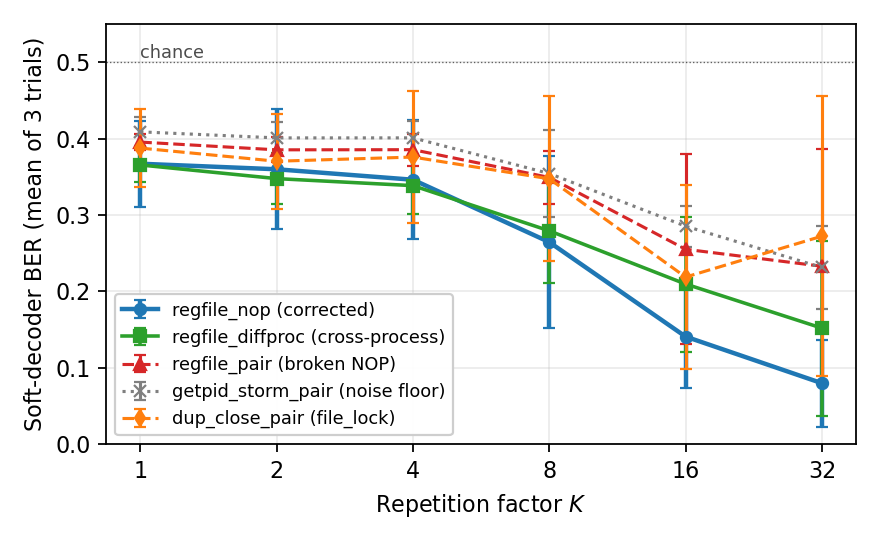
\includegraphics[width=0.98\columnwidth]{ch2_k_sweep.png}
\caption{Repetition $K$-sweep across the five attribution binaries. Each point is the soft-decoder BER averaged over three trials of $1024$ symbol windows}
\label{fig:ksweep}
\end{figure}

\begin{table*}[t]
\centering\small
\caption{Repetition-coding $K$-sweep across the five attribution binaries (mean of $3$ trials, soft-decoder BER). Schedule: $16$ information bits $\times$ $\code{MAX\_K}=32$ $\times$ $\code{LOOPS}=2$ $= 1024$ symbol windows of $50$ ms at $I=200$, sender CPU $1$, receiver CPU $2$, sender SQPOLL CPU $3$, receiver SQPOLL CPU $4$.}
\label{tab:repk}
\begin{tabular}{lcccccc}
\toprule
Variant & $K=1$ & $K=2$ & $K=4$ & $K=8$ & $K=16$ & $K=32$ \\
\midrule
\code{regfile\_nop} (corrected receiver)        & $0.367$ & $0.360$ & $0.346$ & $0.265$ & $0.141$ & $\mathbf{0.080}$ \\
\code{regfile\_diffproc} (cross-process)        & $0.366$ & $0.348$ & $0.339$ & $0.279$ & $0.210$ & $0.152$ \\
\code{regfile\_pair} (legacy, broken receiver)  & $0.396$ & $0.385$ & $0.386$ & $0.349$ & $0.255$ & $0.233$ \\
\code{getpid\_storm\_pair} (syscall noise floor)& $0.409$ & $0.401$ & $0.401$ & $0.354$ & $0.285$ & $0.231$ \\
\code{dup\_close\_pair} (\code{file\_lock} fingerprint) & $0.388$ & $0.370$ & $0.376$ & $0.347$ & $0.219$ & $0.272$ \\
\bottomrule
\end{tabular}
\end{table*}

Figure~\ref{fig:ksweep} plots $K$-vs-BER curves and Table~\ref{tab:repk} reports the underlying numbers for each of the five binaries in our falsifier set. The \code{regfile\_nop} BER falls $4.6\times$ from $0.367$ at $K = 1$ to $0.080$ at $K=32$. One of the three trials reaches zeros errors on 32 super-symbols. At $W = 50$ms and $K=32$ this has throughout $0.625$ bits/sec.

\subsection{Attribution}
\label{sec:ch2attribution}
We can see from the falsifier data that ultimately the \code{refcnt} of the shared file descriptor to \code{/dev/null}. We note also that \code{regfile\_diffproc}--- which is the test in which the sender and receiver open separate kernel objects for \code{/dev/null}--- performs well, reaching $K=32$ soft BER of $0.152$ which is below the noise floor of \code{getpid\_storm\_pair} but above that of \code{regfile\_nop}. This is evidence of two facts. The dominant carrier in \code{regfile\_nop} is the shared \code{struct file} of \code{/dev/null}. This is evident since \code{regfile\_nop} performs better than \code{regfile\_diffproc}. Secondly, there exists a secondary carrier that survives when no \code{struct file} is shared. Cross-process, the only kernel resource the two rings provably share is global allocator state: the \code{kmalloc-32} partial-list locks, per-NUMA \code{zone->lock}, and per-CPU \code{pcp\_lock} of mechanism (c).

This is also where Channel II touches hardware most directly. The carrier of (d) is ultimately MESI traffic on a single cache line, but the sender is provoking this with only user-visible \iouring primitives. We treat this carefully since the magnitude of the signal is set by the cross-CPU coherence penalty of the underlying hardware.

\section{Channel III: Cross-Ring CQE Delivery}
We wonder here if it is possible for a covert channel to exist when neither \code{ATTACH\_WQ} nor a shared \code{struct file} is available and the rings are isolated. It turns out that a documented opcode is apart of modern versions of \iouring with intended use for cross-ring asynchronous communication. We, thus, offer a channel, simply to say that a system administrator should prevent this opcode, \code{IORING\_OP\_MSG\_RING}, on multi-tenant mutually distrustful systems.

\subsection{Mechanism}
\code{IORING\_OP\_MSG\_RING} takes a target ring file descriptor and posts a CQE on that target ring \cite{axboe_msg_ring}. Interanlly, \code{io\_msg\_ring\_data} (in \code{io\_uring/msg\_ring.c}) acquires the target context's \code{completion\_lock}, fills out a CQE, and wakes the target's wait list if needed. From the target's point of view, a CQE has appeared on its CQ ring without any SQE having been submitted itself.

The receiver's per-window probe loop drives the channel. When the sender is storming \code{MSG\_RING} at target \code{receiver\_ring\_fd}, we see three things happen. We first drain any inbound \code{MSG\_RING} delivery CQEs already in the receiver's CQ ring. We, then, allow for the recveiver's subsequent reap to return immediately because a fresh \code{MSG\_RING} CQE is already there. It then consumes the CQE instead of waiting for its \code{NOP} CQE. Third, the iteration count per 50 ms window jumps from $\approx 12000$ in bit-0 windows to $\approx 22000$ in bit-1 windows. LDA on \code{samples} picks this out trivially.

\subsection{Emperical results}
We ran \code{msg\_ring\_pair} for three trials at $W = 50$ ms, $I = 200$, \code{LOOPS} $=2$, $K = 1$, decoded with the same LDA pipeline as before. Per trial $K = 1$ hard BERS were $0.0077$, $0.0000$, and $0.0154$, giving a mean of $0.008 \pm 0.008$. We have a wall-clock throughput of $\approx 18.1$ bits/sec at $K = 1$. The $K = 1$ BER alone is an order of magnitude lower than \code{regfile\_nop} ($\approx 0.367$) and considerably better than the single-ring \code{attached\_pair} cell at $W = 100$ms ($\approx 0.14$). 

\subsection{Adjacent cross-ring opcodes}
We also tested two adjacent cross-ring opcodes that do not go through \code{MSG\_MSG}.

The first is \code{buffer\_register\_pair}, which streams \code{IORING\_OP\_READ\_FIXED} of \code{/dev/null} plus \code{IORING\_REGISTER\_BUFFER\_UPDATE} on the sender with the receiver also doing \code{READ\_FIXED}. Its $K=1$ BER is $0.422 \pm 0.043$. The receiver's \code{vfs\_read} cost dominates, so it is largely insensititive to the buffer-resource churn.

The second is \code{openat\_close\_pair} which streams \code{IORING\_OP\_OPENAT} and \code{IORING\_OP\_CLOSE} on \code{/dev/null} on the sender, with the receiver simply doing \code{OP\_NOP}s. Its $K = 1$ BER is $0.461 \pm 0.014$, also indistinguishable from chance. This is simply because the receiver has no file descriptor touching operation in its hot path. 

These indicate that a cross-ring opcode must have some ability to manifest as a quantity that the hot path observes.

\section{Defenses and Mitigations}
The defenses appropriate to each channel's layer of attacker capability differ in both scope and in which maintainer would be responsible for them. We list four options that are specific to the channel. We do not have full performance measurements for any of them, but each is within scope for future work.

\paragraph{Channel I: deny \code{ATTACH\_WQ} across security domains.} \code{IORING\_SETUP\_ATTACH\_WQ} is the only flag at ring-creation time that opts into shared \code{SQPOLL} backends. A seccomp-bpf or LSM policy can block this flag on \code{io\_uring\_setup} for processes outside of a single trust domain. This is likely the cheapest defense, since it only limits the efficiency of \code{SQPOLL} performance for legitimate multi-ring applications. We claim that a per-cgroup or per-uid exemption is straightforward.

\paragraph{Channel II: prevent shared \code{struct file} across trust domains.} Channel II is dominantly carried by the per-\code{struct file} atomic refcount cache line. The cleanest mitigation thus is to ensure that two rings in mutually distrustful sandboxes cannot register file descriptors that resolve to the same backing \code{struct file}. Mount-namespace separation already blocks the common case, but any LSM that mediates \code{IORING\_REGISTER\_FILES} can also enforce a uniqueness predicate. The residual cross-process signal we measure in \code{regfile\_diffproc} is delivered by global allocator pressure and therefore is not addressed by this defense.

\paragraph{Channel II: per-context memory pool for \code{io\_rsrc\_node\_alloc}.} A patch to \code{io\_uring/rsrc.c} could draw \code{io\_rsrc\_node} from a per-ctx mempool sized to \code{IO\_NODE\_ALLOC\_CACHE\_MAX} which the \code{io\_uring} task-work infrastructure already does for adjacent small structs. This would remove the dependency on the global \code{kmalloc-32} partial list, limiting the \code{regfile\_diffproc} residual signal.

\paragraph{Channel III: block \code{IORING\_OP\_MSG\_RING}} \code{IORING\_OP\_MSG\_RING} is a documented cross-ring primitive that is, by design, to allow communication between rings. The defense is thus simply to disallow this at the policy layer by refusing to allow a \code{MSG\_RING} SQE whose target ring's owning task is in a different sandbox. As with the first mitigation, this can be implemented with eBPF or LSM \cite{he2023ringguard}.

\section{Related Work}
\paragraph{Storage-side covert channels in \code{io\_uring}.} The closest prior work is that found in \textit{Secret Spilling Drive} \cite{juffinger2025secret}, which finds that unprivileged \iouring can saturate the PCIe bus and provoke a measurable timing side channel in a co-resident victim's SSD reads. Our work is complementary to this since their channel runs through the storage device and ours runs through the runtime above the block layer. 

\paragraph{Cache and CPU-internal side channels.} \textsc{Flush+Reload} and the last-level cache attacks of Liu et al. \cite{yarom2014flushreload, liu2015lastlevel} directly module cache-line state between an attacker and a victim in a very similar manner to our Channel II attack. The carrier of both attacks is the MESI traffic of a cache line. In fact, work has been done to make use of this for covert communication with cross-VM caches \cite{maurice2017hello, ristenpart2009hey,wu2014whispers}. Our work, of course, uses the \iouring user-visible primitives to carry out covert communications, while theirs relies, at least in some part, on the ability to issue \code{clflush} or to arrange cache-set conflicts.

\paragraph{Kernel-runtime monitoring.} \textsc{RingGuard} \cite{he2023ringguard} proposes an eBPF-based monitoring layer for \iouring that is aimed at detecting suspicious patterns of opcode use. This would be perfect our proposed mitigations, and it remains future work to implement it as such.

\paragraph{Information theoretics.} The theory behind repetition coding and capacity that we describe in Section~\ref{sec:background} is rather textbook \cite{shannon1948mathematical, cover2006elements}. We direct interested readers towards more knowledgable sources, and we make no claims of information-theoretic optimality. In fact, we only make the claim of existence.

\section{Discussion}
\subsection{Limitations}
We note that all experiments were ran on one Intel Core i7-8650U laptop. Replication on other forms of hardware remains future work. However, it is likely that hardware that is not as noisy as this machine should push \code{SQPOLL}'s noise floor down and create a better opportunity for Channel I. This hardware is also single-NUMA and a multi-socket Xeon to test the cross-NUMA also remains future work. We expect that it might reduce the residual capacity of the \code{regfile\_diffproc} performance.

\subsection{Future work}
Our propositions of the most important future work endeavours is as follows.

\paragraph{Capacity-approaching codes.} Replacing repetition with a soft-decision LDPC or polar code for Channel II could improve the throughput by drastic amounts. If this can be done, especially in regards to \code{regfile\_diffproc}, the result would be most interesting.

\paragraph{Multi-Socket NUMA.} If we pin the sender to socket $0$ and the receiver to socket $1$, we can test cross-NUMA performance for Channel II. We predict, as we said just earlier, that the cross-NUMA penalty might reduce the residual capacity and allow our mitigation to be better scoped.

\paragraph{An \code{io\_rsrc\_node} mempool patch.} A mempool patch, as discussed in the mitigations, could close Channel II at the (c)-mechanism level.

\subsection{Course goals achieved}
We claim that we fully achieved our $100\%$ goal of creating amd verifying the existence of a covert channel in the runtime--- in fact, we produced three of them. We also partially achieved the $125\%$ goal of mitigation strategies by introducing some potential ideas, but we have not tested them, and leave that as future work.

\section{Conclusion}
We demonstrated that \iouring's runtime has at least three distinct covert timing channels, and we organized them according to teh amount of shared kernel state required of the cooperating adversarial processes. With \code{ATTACH\_WQ}, a single shared \code{SQPOLL} kernel thread is enough to deliver a BER near zero at $\approx 86$ bits/sec, and we attribute this directly to the kthread's per-pool inner loop. With independent \code{SQPOLL} backends, but a shared backing \code{struct file}, the per-\code{struct file} atomic refcount cache liner carries a $p = 0.37$ binary symmetric channnel that repeition coding turns into a usable channel but at bits/sec rates at $< 1$ bits/sec. We also note a primitive that \iouring includes that allows for a very simple channel with \code{MSG\_RING}.

We also provide potential avenues for mitigation such as restricting \code{ATTACH\_WQ}, sandboxing file descriptor uniqueness, and disallowing \code{MSG\_RING} for sensitive systems. 
\bibliographystyle{plain}
\bibliography{refs}

\end{document}